\chapter{Monte Carlo Radiation Transport Technique}
\label{sec:mcrt}
\section{Introduction}
This chapter will provide an overview of the Monte Carlo radiation transport method (MCRT) method and compares it to other light transport methods. 
Details of the \gls*{mcrt} code developed during this project and used as the basis of the results reported in subsequent chapters, validation of code, and details of computational speed up are also presented.

\section{Monte Carlo Radiation Transport Algorithm}

\subsection{Introduction and Background}
The technique that makes up the bulk of this thesis is the \gls*{mcrt} technique. This method was developed at the end of the Second World War at the Los Alamos National Laboratory, for the purpose of calculating neutron diffusion through shielding material~\cite{montybeg1,eckhardt1987stan,anderson1986metropolis,ulam1947statistical}. It has since found a myriad of applications from light transport through dusty galactic clouds~\cite{wood1999model}, calculating doses for radiotherapy~\cite{rogers1995beam} to light transport through tissue~\cite{1stmonty}.

The theory that governs the transport of radiation through a medium is the \gls*{rte}.
Before describing~\gls*{mcrt} which is a numerical simulation of the~\gls*{rte}, the theory of radiation transport must be examined.

\subsubsection*{Radiative Transfer}
Transport of radiant energy through turbid media can be modelled analytically using the \gls*{rte}. The \gls*{rte} models the radiative losses and gains by a beam of radiation as it propagates, including: loss of energy due to absorption, loss/gain of energy due to scattering, and energy gain due to emission. Before deriving the \gls*{rte}, definitions of some terms and physical quantities is required.


The first term is spectral irradiance, $L_\nu$. Spectral irradiance is defined as the energy flow in a direction $\mathbf{\hat{n}}$, for a solid angle $d\Omega$, per unit time per unit temporal frequency bandwidth.	
Irradiance is defined as the spectral irradiance over a small frequency range $[\nu, \nu+\Delta \nu]$:

\begin{equation}
	L(\vec{r},\hat{s},t) = L_{\nu}(\vec{r},\hat{s},t)\Delta \nu	
\end{equation}

\noindent Where:

\indent $\vec{r}$ is the position;

\indent $\hat{s}$ is the unit normal vector;

\indent $t$ is the time;

\indent and $L(\vec{r},\hat{s},t)$ is the irradiance [$W\ m^{-2}\ sr^{-1}$].

\medskip

\begin{figure}[!htbp]
	\centering
	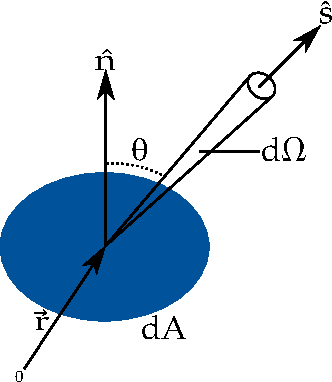
\includegraphics[scale=1.]{diffelement.pdf}
	\caption{Energy flow through area $dA$ within solid angle $d\Omega$ in a direction $\hat{s}$. Adapted from~\cite{wang2012biomedical,chandrasekhar2013radiative}.}
	\label{fig:energydiag1}
\end{figure}

The irradiance can be used to determine the energy, $dE$, transported across an area $dA$, in a solid angle $d\Omega$ in a time $dt$ (see~\cref{fig:energydiag1}) is:

\begin{equation}
	dE = L(\vec{r},\hat{s},t) \cdot cos\left(\theta\right)\ dA\ d\Omega\ dt
\end{equation}

\noindent Where:

\indent $\hat{n}$ is the unit normal to $dA$;

\indent and $cos\left(\theta\right)$ is the angle between $\hat{n}$ and $\hat{s}$.

\medskip

Irradiance can also be used to determine the fluence rate, $\phi$, which is defined as the energy flow per unit time, independent of the flow direction.

\begin{equation}
	\phi(\vec{r},t)=\int_{4\pi}L(\vec{r},\hat{s},t)\ d\Omega
\end{equation}

\noindent Where:

\indent $\phi$ is the fluence rate [$W m^{-2}$].

\medskip

Solving the \gls*{rte} yields the irradiance which gives the distribution of light in the medium, information on the state of the system, and all the physical properties of it.

With the irradiance defined, as well as the other quantities that follow, the \gls*{rte} can be derived~\cite{chandrasekhar2013radiative,wang2012biomedical}. First considering the conservation of energy, as shown in~\cref{eqn:enegyconvo}.

\begin{equation}
	dP = -dP_{div} - dP_{ext} + dP_{scatt} + dP_{src}
	\label{eqn:enegyconvo}
\end{equation}

\noindent Where:

\indent $dP$ is the total change in energy in the volume $dA\ ds$ within the solid angle, $d\Omega$, per unit 

\indent time (see~\cref{fig:energydiag2});

\indent $dP_{div}$ is the energy loss due to the divergence of the radiation beam per unit time;

\indent $dP_{ext}$ is the energy loss due to absorption and scattering within the volume $dA\ ds$ within the

\indent  solid angle, $d\Omega$;

\indent $dP_{scatt}$ is the energy gain due to scattering from $\hat{s}'$ into $d\Omega$ per unit time;

\indent and $dP_{src}$ is the energy gain due to emission within the medium, per unit time.

\medskip

The total change in energy, $dP$, in the volume element within the solid angle $d\Omega$ is equal to:

\begin{equation}
	dP=\frac{1}{c}\frac{\partial L(\vec{r},\hat{s},t)}{\partial t}\ dA\ ds\ d\Omega
	\label{eqn:p}
\end{equation}

\noindent Where c is the speed of light.

\medskip

\begin{figure}[!htbp]
	\centering
	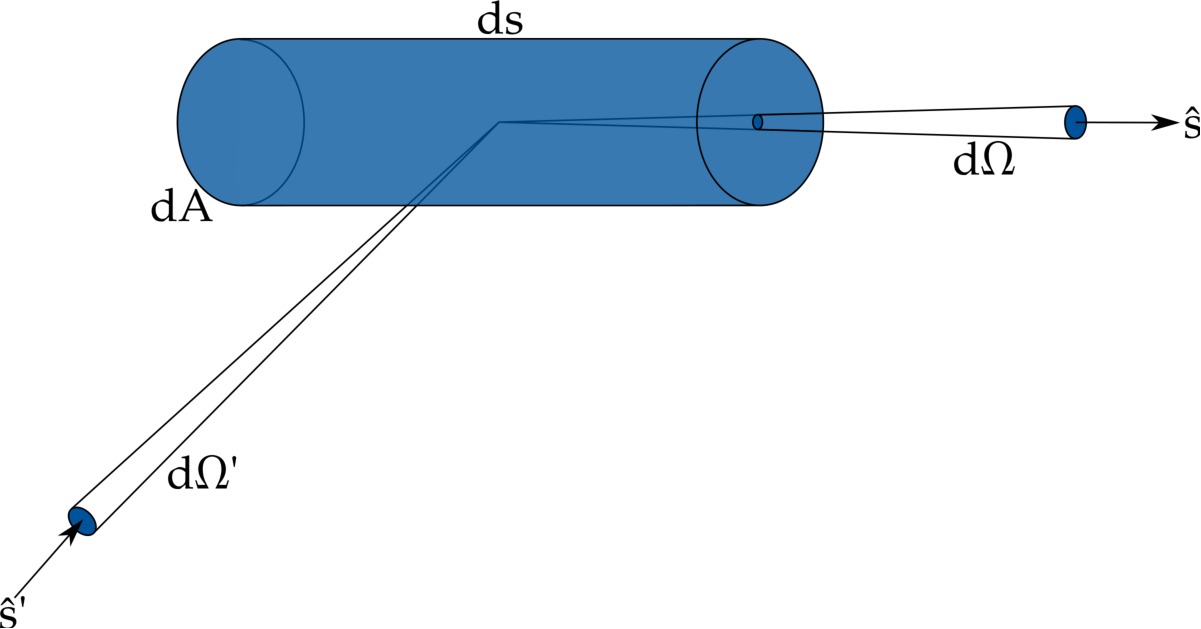
\includegraphics[scale=0.5]{cylinderelement.pdf}
	\caption{Cylindrical volume element, $ds\ dA$, with solid angle $d\Omega$ in direction $\hat{s}$ and solid angle $d\Omega'$ in direction $\hat{s}'$. Energy flowing through this element is used to derive the radiation transfer equation. Adapted from~\cite{wang2012biomedical,chandrasekhar2013radiative}.}
	\label{fig:energydiag2}
\end{figure}

The first loss term, $dP_{div}$, is the energy loss due to divergence of the radiation beam. This is modelled as:

\begin{align}
	dP_{div}&=\frac{\partial L}{\partial s}\ d\Omega\ dV \\
		    &=\hat{s} \cdot \nabla L(\vec{r},\hat{s},t)\ d\Omega\ dV
    \label{eqn:pdiv}
\end{align}

$dP_{ext}$ is the second loss term, and accounts for energy loss due to scattering and absorption in the volume element within the solid angle $d\Omega$. This is modelled as:


\begin{equation}
	dP_{ext}=\mu_t ds\ L(\vec{r},\hat{s},t)\ dA\ d\Omega
	\label{eqn:pext}
\end{equation}

Where $\mu_t$ is the extinction coefficient [$m^{-1}$], see \cref{sec:optprop} for further details.

The first energy gain term, $dP_{src}$, is due to emission in the volume element within the solid angle $d\Omega$ from a source, $S(\vec{r},\hat{s},t)$ [$Wm^{-3}sr^{-1}$]. 

\begin{equation}
	dP_{src}=S(\vec{r},\hat{s},t)\ dV\ d\Omega
	\label{eqn:psrc}
\end{equation}

The second energy gain term, and final term, is due to the incident energy on the volume element within the solid angle $d\Omega$ in direction $\hat{s}$ due to scattering from any direction $\hat{s}'$.

\begin{align}
	dP_{scatt}&=N_sdV\left(\int_{4\pi}L(\vec{r},\hat{s}',t)P(\hat{s}',\hat{s})\sigma_s\ d\Omega' \right)\ d\Omega \\
			  &=\mu_sdV\left(\int_{4\pi}L(\vec{r},\hat{s}',t)P(\hat{s}',\hat{s})\ d\Omega' \right)\ d\Omega 
			  \label{eqn:pscatt}
\end{align}

\noindent Where:

\indent $N_s$ is the number density of scatterers [$\#m^{-3}$];

\indent $P(\hat{s}',\hat{s})$ is the scattering phase function (see~\cref{sec:optprop} for further discussion);

\indent and $\sigma_s$ is the cross section of the scatterers [$m^2$], thus $\mu_s=N_s\sigma_s$, where $\mu_s$ is the 

\indent scattering coefficient [$m^{-1}$].

\medskip


Finally substituting~\cref{eqn:pext,eqn:psrc,eqn:pdiv,eqn:pscatt,eqn:p} into~\cref{eqn:enegyconvo} yields the \gls*{rte}:

\begin{equation}
\frac{1}{c}\frac{\partial L(\vec{r},\hat{s},t)}{\partial t} + s\cdot \nabla L(\vec{r},\hat{s},t)=-\mu_tL(\vec{r},\hat{s},t)+\mu_s\int_{4\pi}p(\hat{s},\hat{s}')L(\vec{r},\hat{s}',t)\ d\Omega' + S(\vec{r},\hat{s},t)
\label{eqn:rte}
\end{equation}


In general, the \gls*{rte} is hard to solve in arbitrary 3D geometries, however there are several approximations, and numerical methods available. The diffusion approximation, \gls*{km}, and \gls*{mcrt} are the common methods used to approximate or solve the \gls*{rte}.
This section discusses in brief each of these methods and their respective pitfalls, and positive aspects.

\subsubsection*{Kubelka-Munk Theory}
\gls*{km} was originally developed to calculate the light distribution in thin layered materials, such as paint or paper~\cite{barbaric2011kubelka}. The theory is rather simple and makes many assumptions about the medium and the incident light. The main assumptions of \gls*{km} are: only scattering and absorption take place in the medium, the incident light is already diffuse, the medium is uniform with only isotropic scattering, no external or internal reflections, and the medium is planar and infinitely wide~\cite{jasinski2011modelling,cheong1990review,gabriela2013mathematical}.

These assumptions make \gls*{km} poor for modelling light-tissue interactions.
This is because in tissue, scattering is not isotropic but rather forward biased (see~\cref{sec:optprop}). 
Tissue is rarely, planar and infinitely wide. 
Tissue also has some reflections at its external and internal boundaries, due to changes in refractive indices. 
Many medical and biophotonic treatments/methods use laser light which is not diffuse. Finally, tissue can also exhibit fluorescence, which the \gls*{km} is not able to model, along with polarization. 
\gls*{km} does have some positive aspects.
\Gls*{km} theory is good at calculating the diffuse reflectance of simple media, and can be used to roughly estimate calculations. Though it is not well suited for modelling light-tissue applications~\cite{prahl1990light}.

\subsubsection*{Diffusion Approximation}
\label{sec:diffusionapprox}
The diffusion approximation for the \gls*{rte} is where the irradiance is separated into two components:

\begin{equation}
	L(\vec{r},\hat{s}) = L_c(\vec{r},\hat{s}) + L_d(\vec{r},\hat{s})
\end{equation}
Where $L_c$ is the unscattered contribution, which satisfies Beer's law\footnote{Beer's law (or Beer-Lambert law) states that the transmission, $T$, is equal to $e^{-\mu L}$, where $L$ is the distance and $\mu$ is the attenuation coefficient.}, and $L_d$ is the diffuse contribution. The $L_d$ component is expanded using Legendre polynomials and truncated. 
The diffusion approximation also has several assumptions and restrictions. The main assumption is that scattering dominates over absorption, and that the scattering is nearly isotropic. This restricts the types of scattering the diffusion approximation can model, though using similarity relations can partially model scattering in tissue~\cite{graaff1993similarity,yoon1989accuracies}.

The diffusion approximation is computationally fast, and simple to implement. However, it is poor at modelling light-tissue interactions due to its assumptions and restrictions, mainly the inaccurate modelling near the boundaries of the medium and its lack of modelling fluorescence and other microphysics. Though it can be used to speed up \gls*{mcrt} in mediums where scattering dominates~\cite{robitaille2010modified,min2009radiative}.

\subsubsection*{MCRT}
The final method, \gls*{mcrt}, is numerically equivalent to the \gls*{rte}~\cite{wang2012biomedical}. \gls*{mcrt} is a flexible method, it can model arbitrary 3D geometries, various microphysics including fluorescence and polarisation.
\Gls*{mcrt} can also model various different light sources, from collimated laser beams to diffuse light sources. The only downside noted in the literature is that the \gls*{mcrt} can be expensive computationally. However, with computational power growing faster with time, this is less of a problem going forward. 

The next several sections give an in depth description of the \gls*{mcrt} method and its flexibility, along with a description of the code used in this thesis to solve various medical and biophotonic problems.

\subsection{Optical Properties}\label{sec:optprop}

Before an in-depth description of the \gls*{mcrt} method is outlined, a discussion of the optical properties of materials is presented, which the \gls*{mcrt} method requires to simulate the transport of photons in a medium.

Optical properties of a medium are the properties that describe how light is transported through that medium. Usually the optical properties of a medium are defined by three main parameters: the scattering ($\mu_s$), anisotropy ($g$), and  absorption ($\mu_a$) coefficients.

\subsubsection*{Scattering}\label{sec:scatt}

The scattering coefficient, along with the anisotropy value (see~\nameref{sec:ansio}), define how light is scattered in a medium. The main scatterers in the deeper layers of the skin are filamentous proteins such as collagen and elastin~\cite{jacques1996origins}. In the upper layers of the skin, the main scatterers are keratins and various chromophores such as melanin. 
The size of the scatterers affect how light is scattered and into which direction that light is scattered into.

\medskip

The scattering of light within tissue is usually defined as $\mu_s$ or $\mu_s'$: the scattering coefficient and the reduced scattering coefficient, where $\mu_s'=\mu_s(1-g)$. The scattering coefficient is defined such that the probability of transmission without scattering and neglecting absorption in a path length L is:

\begin{equation}
	T=e^{-\mu_sL}
\end{equation}
This gives units of inverse length for the scattering coefficient (usually measured in $cm^{-1}$ in medical applications). The reduced scattering coefficient is often given in place of the scattering coefficient, as the reduced coefficient is more easily measured then the ``normal'' coefficient~\cite{jacques2013optical}.



\subsubsection*{Anisotropy}\label{sec:ansio}

Anisotropy is the degree of deviation that light undergoes at each scattering event. The anisotropy value is taken from the phase function for the medium. The phase function is defined as the angular distribution of light intensity scattered by a particle. The phase function, $\Phi(\theta,\phi)$, is usually normalised over all angles:

\begin{equation}
	\int_{\Omega}\Phi(\theta,\phi)\ d\Omega = 1
\end{equation}

Where $\theta$, and $\phi$ are the usual polar and azimuthal spherical angles, and $d\Omega=\sin\theta d\theta d\phi$.
Thus, for Rayleigh and isotropic scattering, their phase functions are:

\begin{align}
	\Phi_{isotropic}(\theta,\phi)&=\frac{1}{4\pi}\\
	\Phi_{Rayleigh}(\theta,\phi)&=\frac{3}{8\pi}(1+cos^2(\theta))
\end{align}

For simplicity, the phase function is usually cast as the anisotropy value g, which is defined as the average angle of deflection:

\begin{equation}
	g=\left<cos(\theta)\right>=\int_{\Omega}\cos\theta\ \Phi(\theta,\phi)\ d\Omega
\end{equation}
The anisotropy factor, g, can take on any value from $-1$ to $1$. Where a value of $-1$ is totally back scattering, $0$ is isotropic scattering, and $1$ is totally forward scattering (see~\cref{fig:henyey}).

\begin{figure}[!htbp]
	\centering
	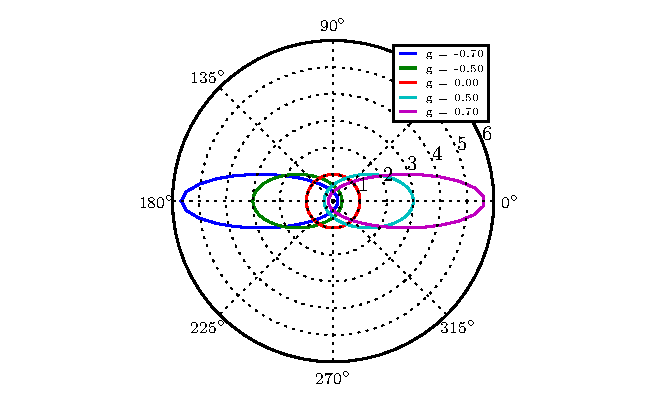
\includegraphics[width=.75\textwidth]{polar.pdf}
	\caption{Figure shows the g factor for the Henyey-Greenstein phase function, for various configurations of back, forward or isotropic scattering. Arrow indicates the photons initial direction before scattering.}
	\label{fig:henyey}
\end{figure}
There are many phase functions that can be used to model the anisotropy factor in a medium. The standard phase function in biological tissue is the Henyey-Greenstein phase function. The Henyey-Greenstein phase function, was originally created to model scattering of diffuse radiation in the galaxy~\cite{lister2012optical,henyey1941diffuse}. It has since become the \textit{de-facto} phase function for biological tissue. This is due to the phase functions relative simplicity and due to it being regarded as a ``good'' phase function for approximating scattering in biological tissue~\cite{jacques1987angular}.
The Henyey-Greenstein phase function is shown in~\cref{eqn:henyey}:

\begin{equation}
	\Phi_{H.G}(\theta,\phi)=\frac{1}{4\pi}\frac{1-g^2}{(1+g^2-2g\ cos(\theta))^{\tfrac{3}{2}}}
	\label{eqn:henyey}
\end{equation}

The Henyey-Greenstein phase function will be adopted as the phase function for the whole of this thesis.

\subsubsection*{Absorption}\label{sec:absor}

Absorption of light by a medium is defined by the absorption coefficient $\mu_a$. The absorption coefficient is defined in a similar fashion to the scattering coefficient, by considering the probability of transmission without absorbing and neglecting scattering in a path length L:

\begin{equation}
	T=e^{-\mu_aL}
\end{equation}
This, again like the scattering coefficient, gives inverse distance for the unit of the absorption coefficient (and usually measured in units of $cm^{-1}$).

There are various sources of absorbers in tissue including blood, water, fat, melanin, $\beta$-carotene, and bilirubin. These chromophores can all contribute, depending on the wavelength, with some more absorbing than others, as shown in~\cref{fig:absorb}.
The absorbed photons can then be remitted as fluorescence or absorbed as heat. 

\begin{figure}[!htbp]
	\centering
	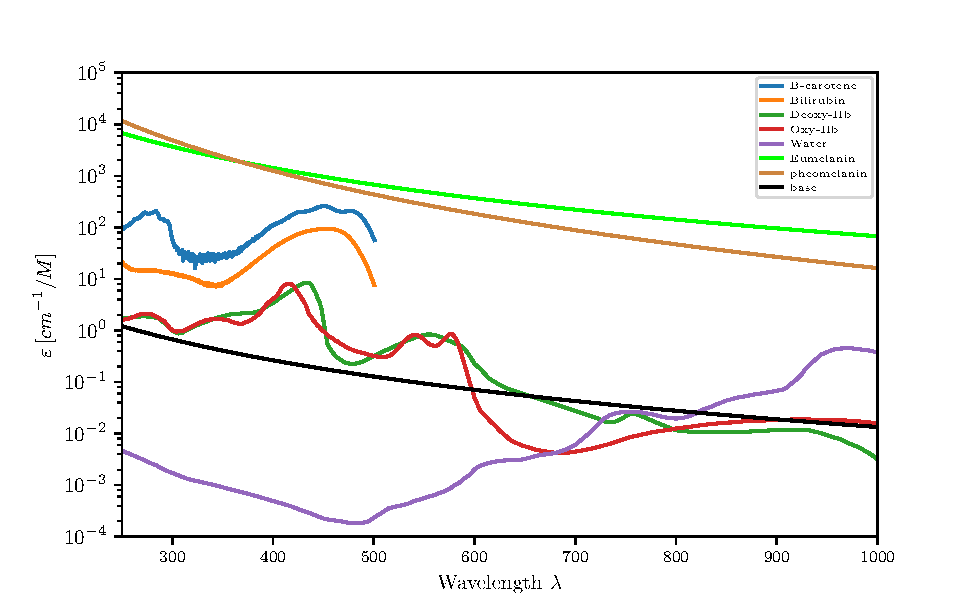
\includegraphics[width=.95\textwidth]{absorbers.pdf}
	\caption{Examples of wavelength dependent absorption coefficients for some common tissue chromophores~\cite{dixon2005photochemcad,photoprahl2017,segelstein1981complex,pope1997absorption,jacques2013optical,van2004determination,saidi1992transcutaneous,iglesias2015biophysically,bashkatov2011optical,sarna2006physical}.}
	\label{fig:absorb}
\end{figure}


\subsubsection*{Derived Parameters}

There are also some derived parameters that are useful to be defined.
These are the albedo and the total attenuation coefficient.

The total attenuation coefficient is defined as the sum of the scattering coefficient and the absorption coefficient:

\begin{equation}
\mu_t=\mu_s+\mu_a
\end{equation}

The albedo, or scattering probability, is defined as the ratio of the scattering coefficient to the total attenuation coefficient:

\begin{equation}
a = \frac{\mu_s}{\mu_a+\mu_s}=\frac{\mu_s}{\mu_t}
\end{equation}


\subsection*{Other Parameters}\label{sec:other}
The preceding subsection described the optical properties that this thesis will use in every chapter. However, there are other optical properties that can be used to define a medium. These other parameters generally are used to model microphysics such as Raman scattering, polarization, fluorescence or reflection/refraction. This section will give a brief overview of these other optical properties.



% \medskip

% \subsubsection*{Refractive Index}
% The refractive index of a medium, defines how fast light propagates through that medium. Generally, for tissue, the refractive index is given as a bulk refractive index. Meaning that the medium is divided into sections, with each section given a refractive index. For example, skin's refractive indices are divided up by the different layers of skin. Details on how refraction is implemented with the code can  be found in~\cref{chap:salvo}.

% \medskip

% \subsubsection*{Raman Scattering}
% Raman scattering is where a photon is scattered inelastically, which excites the molecule the photon scattered off, thus decreasing the energy of the photon and increasing the photons wavelength. 
% The optical property needed to model Raman scattering is the Raman scattering cross section. The cross section, like the absorption or scattering coefficient, is the likelihood of a photon undergoing a Raman scattering event. Raman scattering has been modelled in \gls*{mcrt} in order to simulate spatially offset Raman spectroscopy for breast tumour analysis~\cite{keller2010monte}.

\medskip

\subsubsection*{Fluorescence}



Fluorescence occurs when a photon is absorbed by a fluorescent molecule and re-emitted with a new wavelength. Fluorescence	is a reactively common phenomena, and is heavily utilised in biophotonics and medicine, to image, or monitor molecules in tissue. Again the optical property that models fluorescence is a coefficient that gives the probability of absorption and re-emission of a photon by a certain molecule. Usually this is in the form of an absorption coefficient or extinction coefficient. The extinction coefficient is a measurement of absorption in terms of the concentration of the absorber. Thus, if a medium has many fluorophores, then the total absorption coefficient is the bulk absorption of the medium plus the contribution from the fluorophores as in~\cref{eqn:exct}:

\begin{equation}
\mu_a=ln(10) \sum_i C_i \varepsilon_i
\label{eqn:exct}	
\end{equation}

Where $C_i$ is the concentration of the $i^{th}$ fluorophore, and $\varepsilon_i$ is the extinction coefficient of the $i^{th}$ fluorophore.

Fluorescence will be described in more depth in~\cref{chap:salvo}.
\newpage
\subsection{MCRT Algorithm}\label{sec:algorithmMCRT}

\begin{wrapfigure}{r}{.45\textwidth}
\centering
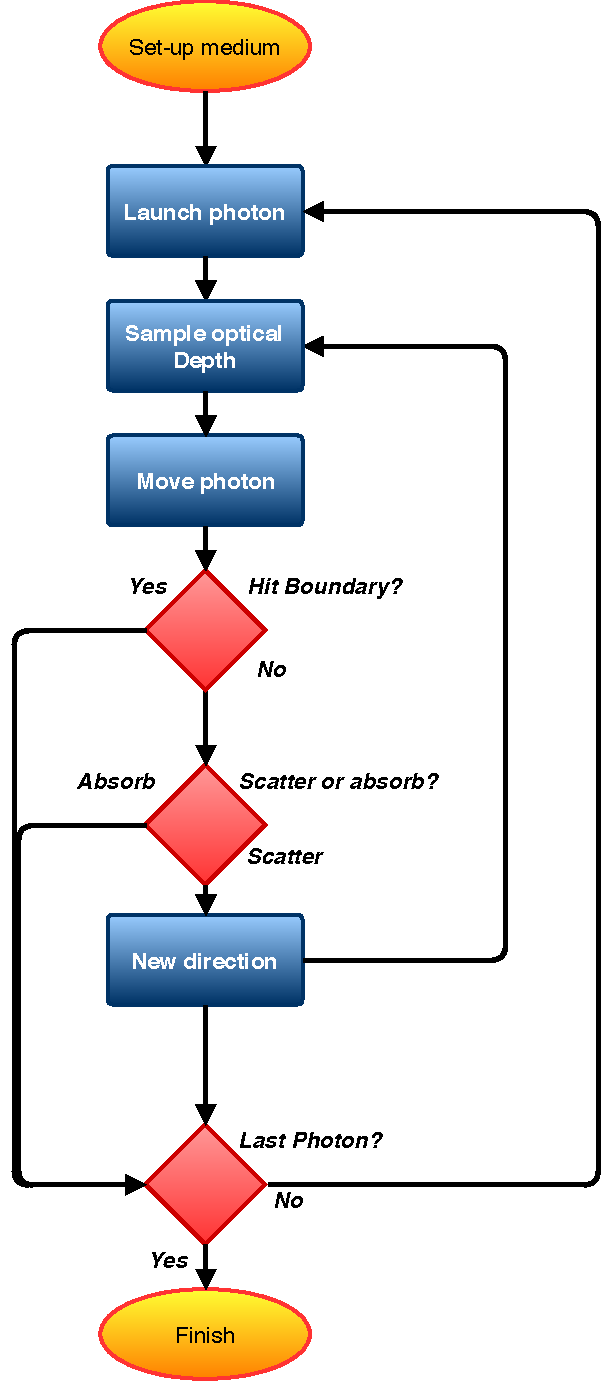
\includegraphics[width=.45\textwidth]{algopic.pdf}
\caption{Flowchart of the Monte Carlo radiation transport algorithm as described in this section.}
\label{fig:algo}
\vspace{-61pt}
\end{wrapfigure}
\FloatBarrier

This section will provide an in depth description of the \gls*{mcrt} algorithm for the propagating photons through a spherical medium with optical properties $\mu_s$, and $\mu_a$. The subsequent section provides details of how the \gls*{mcrt} algorithm is implemented in the Fortran programming language, along with the various code details, such as the parallelisation of the code.

\Cref{fig:algo} shows a flow chart of the~\gls*{mcrt} algorithm described in this chapter.


\subsubsection*{Medium and Grid Set-up}\label{sec:algomedium}
The first step of any \gls*{mcrt} algorithm, is to set-up the medium the photons will propagate through. There are a variety of ways the medium can be set-up. For this section, it is assumed that the medium is an isotropic sphere, radius R, and centred at the origin. For simplicity one wavelength is considered, $\lambda$. As the \gls*{mcrt} algorithm presented here is run on a 3D Cartesian grid, the grid is setup before creating the spherical medium. The grid is composed of $n_x \times n_y \times n_z$ voxels\footnote{A voxel is a 3D pixel}, where each voxel can have its own optical properties.
The grid is setup by first setting an array that stores the locations of the voxel boundary walls in the $x,\ y$, and $z$ directions. 
The next step is to setup the actual medium. This is achieved by discretising the medium onto a grid. 
For this example a sphere is inscribed into a cubic volume, by setting the optical properties of a voxel to that of the medium if the sphere encloses that voxel. The voxels out with sphere are set to that of the ambient medium. An example of a voxelised medium can be seen in~\cref{fig:voxel-model}. 



\subsubsection*{Photon Launch and Initialisation}\label{sec:photlaunch}

The second step in the \gls*{mcrt} algorithm, is to initialise the photon. Initialisation of the photon involves setting its initial position and direction. Again, how this is done depends on the experiment being simulated. Here the photon is initialised to the centre of the sphere. The initial direction is sampled isotropically, and set accordingly:

\begin{align}
n_{xp}&=\sin\theta \cdot \cos\phi \label{eqn:dirvec1}\\
n_{yp}&=\sin\theta \cdot \sin\phi \label{eqn:dirvec2}\\
n_{zp}&=\cos\theta \label{eqn:dirvec3}
\end{align}


With $\theta$ and $\phi$ sampled uniformly between $[0,\ cos^{-1}(2\xi-1)]$ and $[0,2\pi\xi]$ respectively, where $\xi$ is a random number in the range [0,1).

The next step is to launch a photon packet. 
Depending on the source of photon packets for a given simulation, this step varies from simulation to simulation. 
The general idea of launching a photon packet is that the packet is given an initial direction vector and position (which consists of a physical position and a voxel position)\footnote{all variables given in this section are the same as they are in the code.}:

\begin{align}
	direction &= \begin{bmatrix}
		n_{xp}\\
		n_{yp}\\
		n_{zp}
	\end{bmatrix}\\
	position &= \begin{bmatrix}
		x_p, y_p, z_p\\
	\end{bmatrix}\\
	voxel &= \begin{bmatrix}
		x_{cell}, y_{cell}, z_{cell}
	\end{bmatrix}	 
\end{align}

To set the direction vectors, the components of the direction vectors must be first set. The packets position is tracked using a Cartesian coordinate system, however for ease of computation for calculating scattering angles (see~\nameref{sec:photscatterabsorb}), the direction vectors are computed in a spherical system thus the direction vectors are in~\cref{eqn:dirvec1,eqn:dirvec2,eqn:dirvec3}. 

$\theta$ and $\phi$ are generated dependent on the photon source used. The individual sine and cosine terms are saved for use in the scattering routines (see~\nameref{sec:photscatterabsorb}).
The position is then set according to the light source used.
For this example the photons are released from the origin of the sphere.
Using this position the voxel the packet is in is calculated.
\FloatBarrier

\begin{figure}[!htbp]
\centering
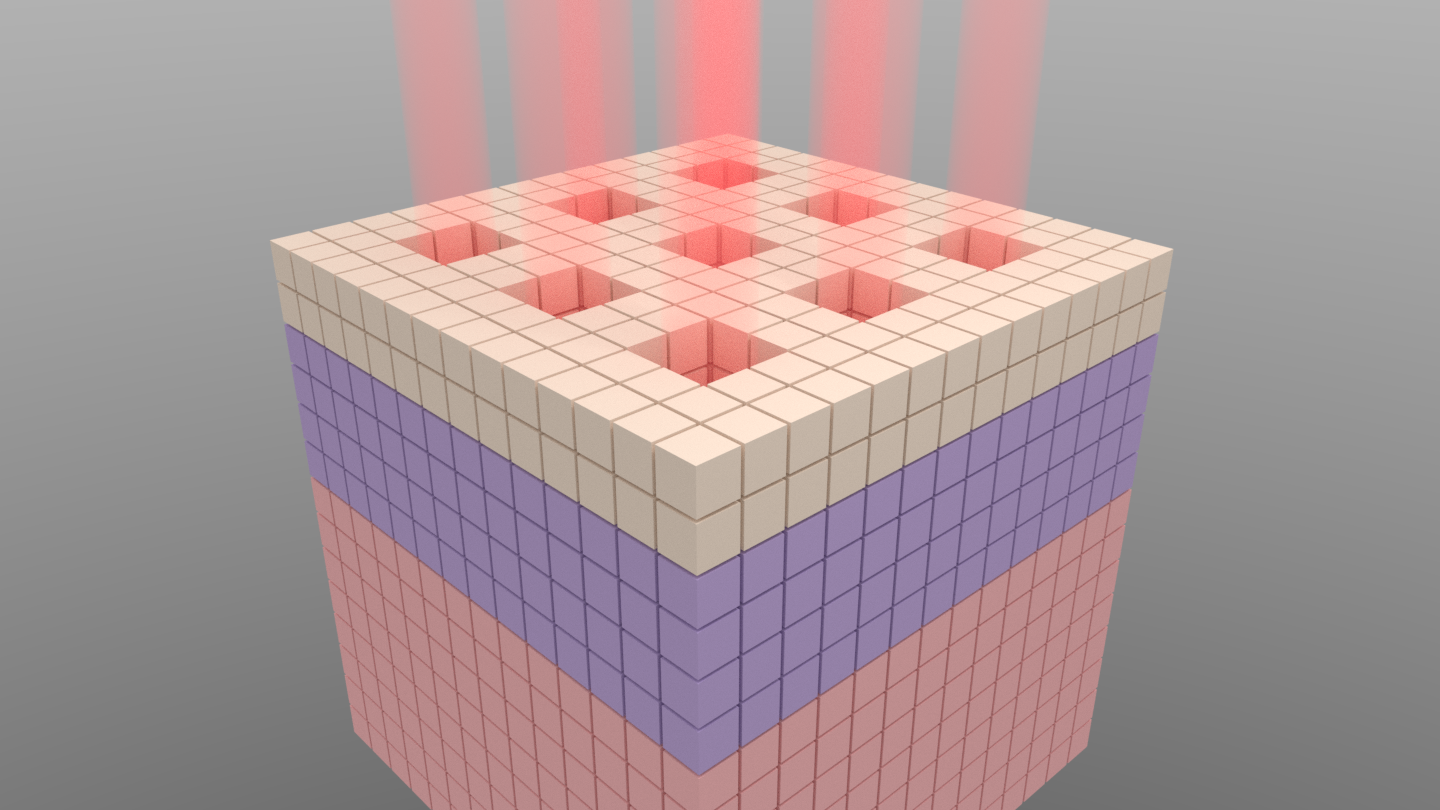
\includegraphics[width=0.5\textwidth]{voxel-model-render.png}
\caption{Example of a possible voxel model, with three different layers, various holes due to ablative pixel beam lasers (~see~\cref{chap:ablation}). Each voxel can represent a different optical/thermal property of the tissue medium.}
\label{fig:voxel-model}
\vspace{-20pt}
\end{figure}
\subsubsection*{Photon Propagation}\label{sec:photmove}

The next step in the algorithm is moving a packet to the next interaction point. The probability that a packet will interact over a distance $dL$ is $\mu_tdL$, where $\mu_t$ is the total extinction coefficient (see~\nameref{sec:optprop}). Thus, the probability of travelling $dL$ without any interaction is $1-\mu_tdL$. Therefore, over a distance $L$ with N segments of length $L/N$ the probability of travelling $L$ before any interaction:

\begin{align}
P(L) &= (1-\mu_t\frac{L}{N}) \cdot (1-\mu_t\frac{L}{N}) ...\ (1-\mu_t\frac{L}{N}) = (1-\mu_t\frac{L}{N})^N \\
P(L) &= \lim_{N \to \infty}(1-\mu_t\frac{L}{N})^N=e^{-\mu_tL}=e^{-\tau}\label{eqn:pdfdist}
\end{align}

Where $\tau$ is the number of mean free paths in a distance L. \cref{eqn:pdfdist} is now a~\gls*{pdf} for the distance a packet will travel before an interaction occurs. To be able to get a random optical depth, the~\gls*{pdf} has to be able to be sampled from either analytically or via the rejection method.
Using the Monte Carlo method described in~\cref{sec:mcmethod}, with $\xi$ as our random number, gives:

\begin{equation}
\xi=\int_{0}^{\tau}e^{-\tau'}=1-e^{-\tau}\rightarrow \tau=-ln(1-\xi)
\end{equation}

As $\xi$ is symmetric about 0.5, $1-\xi$ can be substituted for $\xi$ yielding:

\begin{equation}
\tau=-ln(\xi)\label{eqn:taueqn}
\end{equation} 

$\tau$ is now the optical distance, however this needs to be converted into a physical distance so that the photon packet can be moved. From our definition of $\tau$ we know that $\tau=\int_0^L\mu_tdS$, and if the medium is smooth and homogeneous (i.e not a gridded medium): 

\begin{equation}
L=\frac{\tau}{\mu_t}\label{eqn:physicaldist}
\end{equation}

Therefore, to update the packets position it is simply:

\begin{align}
x_p &= x_p+L\cdot n_{xp}\label{eqn:update1}\\
y_p &= y_p+L\cdot n_{yp}\label{eqn:update2}\\
z_p &= z_p+L\cdot n_{zp}\label{eqn:update3}
\end{align}

However, as the code in this thesis is a 3D gridded Cartesian code, the method of updating and moving the packets position is slightly adjusted. As stated in~\nameref{sec:algomedium}, the medium has been discretised onto a grid, so that each voxel can have a different $\mu_t$, thus~\cref{eqn:physicaldist} becomes:

\begin{equation}
L=\frac{\tau}{\mu_{t,\zeta}}\quad\quad \zeta=(x,y,z)
\label{eqn:voxeloptdist}
\end{equation}

with $\mu_{t,\zeta}$ the attenuation coefficient for the $\zeta^{th}$ voxel. 

\medskip

Moving the photon through a voxelised medium is more involved than propagating a photon through a non voxelised medium. 
This is because the voxel the photon is in needs to be updated as the photon moves from voxel to voxel.
% This is mainly due to the fact the ``book keeping'' needed in tracking where the photon is and in what voxel it is in.
The first step of moving the photon through a voxelised medium is drawing a random optical depth.
This optical depth will be the full optical depth the photon travels before an interaction event.
The generation of a random optical depth is as outlined above, $\tau=-ln(\xi)$.
As the photon travels through the voxel grid, a running total of the current optical distance travelled is kept.
This is then compared to the randomly generated optical depth.
When the running total optical depth equals the randomly generated optical depth the photon propagation is stopped, and the photon undergoes an interaction.

We then calculate the distance to the nearest voxel boundary in the $x,\ y,\ \text{and}\ z$ directions.
The distance is calculated for each direction.~\Cref{eqn:walldist} shows for the $x$ direction:

\begin{equation}
d_{x} = \tfrac{x_{face} - x_{cur}}{n_{xp}}
\label{eqn:walldist}
\end{equation}

Where $d_x$ is the distance to the nearest wall in the $x$ direction. $x_{face}$ is the voxel wall position in the $x$ direction, and $n_{xp}$ is the $x$ direction vector.
With three distances calculated, [$d_x, d_y, d_z$], the minimum of these is thus the distance to the nearest voxel wall.

The next step is to calculate the optical depth for this distance.
The optical depth is found by rearranging~\cref{eqn:voxeloptdist} for $\tau$, with $L$ now the distance to the nearest wall.
With the optical distance to the nearest wall calculated, the next step is to determine if there is ``enough'' optical distance left to travel the full distance to the nearest wall.
Therefore, the running total optical distance is compared to the randomly generated optical distance.
If the running total + the new optical distance to the nearest wall, is less than the randomly generated optical depth, then the photon travels to the nearest wall.
The photon is then placed in the next voxel by a distance $\delta$, where $\delta$ is just larger than machine precision.
If the running total + the new optical distance to the nearest wall is greater than the generated optical distance then an interaction event occurs in the current voxel.
The distance to the interaction event is calculated and the photon moved to this location. 

\Cref{fig:voxelpropexplain} illustrates this whole process for a 2D example.

\begin{figure}[!htbp]
	\centering
	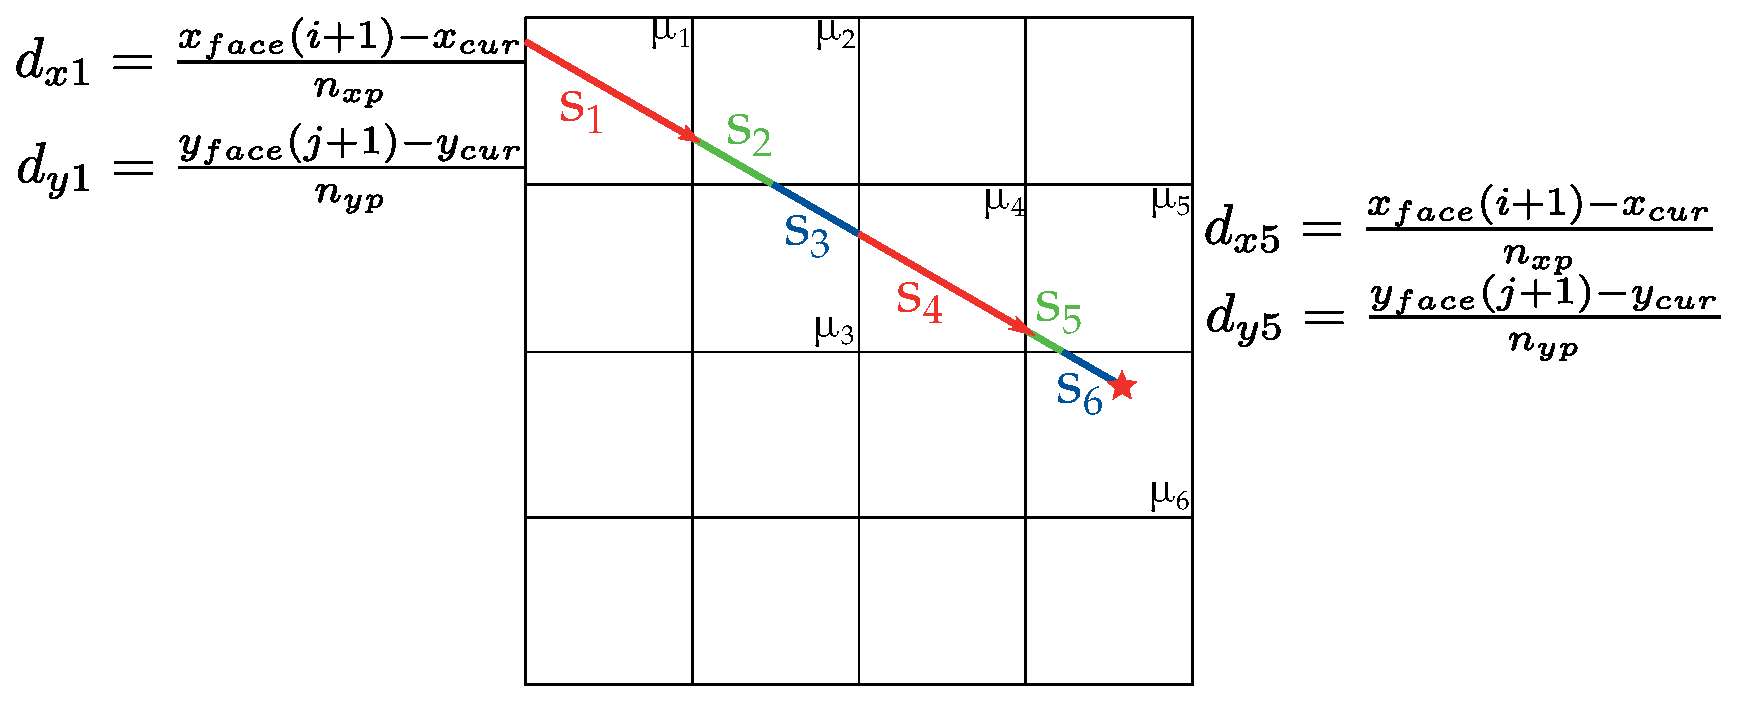
\includegraphics[width=0.75\textwidth]{grid_explain.eps}
	\caption{Illustration of photon propagation through a 2D grid. $d_{x1}$, and $d_{y1}$ are the distances to the voxel walls in the x and y directions in the $\mu_1$ voxel. In this case $S_1=d_{x1}$ as $d_{x1}$ is smaller than $d_{y1}$, thus the photon hits the voxel wall in the $x$ direction. For the $\mu_5$ voxel, $d_y$ is smaller, thus the photon hits the voxel wall in the $y^{th}$ direction.}
	\label{fig:voxelpropexplain}
\end{figure}

This whole process is repeated until the photon undergoes an interaction event or leaves the voxel medium.
The next step in the algorithm is the interaction event, which can consist of either: scattering, absorbing or another microphysics phenomena. 

\subsubsection*{Photon Interaction Event}\label{sec:photscatterabsorb}

The next section of the algorithm is to decide how the photon interacts with the medium, either via scattering or absorption. There are other interaction events that can occur, however descriptions of these are left for the chapters that detail these behaviours.
\medskip

To decide whether a packet scatters or absorbs a random number, $\xi$, is generated and compared against the albedo, $a$. 
If $\xi < a$ then the packet scatters, otherwise it is absorbed. 
% The random number is compared to the albedo, and if the random number is less than the albedo then the packet scatters, otherwise the packet is absorbed.

\paragraph{Packet Absorption}\hspace{0pt}\\
\\
If the interaction event is a photon packet absorption, then the algorithm terminates the photon packets and starts the next photon packet, see~\nameref{sec:terminator}.

\paragraph{Packet Scattering}\hspace{0pt}\\
\\
If the interaction event is a packet scattering, then the packet is scattered into a new direction and the above processes are carried out until a termination clause is met, see~\nameref{sec:terminator}.

Depending on the medium being simulated, it can either be isotropic or anisotropic scattering. 
For the isotropic case, new $cos\left(\theta\right)$ and $\phi$ angles are sampled uniformly, and the direction vectors set as in section~\nameref{sec:photlaunch}.
For the case where the scattering is anisotropic the calculation of the scattering angles, $\theta$ and $\phi$, is more complicated.
The random sampling of the scattering angles, $\theta$ and $\phi$, are valid in the ``centre of mass'' frame containing the scatter, incident and scattered ray.
The photons position is updated in the lab frame, thus the direction vectors also have to be updated in the lab frame.
This means that the scattering angles need to be rotated into the lab frame.
For the isotropic case we assume that the scattering is also isotropic in the lab frame, thus the new direction vector is easily calculated.
However, this is not the case for anisotropic scattering, as the centre of mass frame has to be rotated into the lab frame.

\medskip

\Cref{fig:labframerotate} and~\cref{eqn:scatrotate} show how this process is achieved.
Where $\mathbf{n}=(n_x,n_y,n_z)$, $\mathbf{n_s}=(n_{x}^{new},n_{y}^{new},n_{z}^{new})$, $\theta_s$ is chosen from the phase function~\cref{eqn:henyeysample}, and $\varphi_s=2\pi \xi$ with $\xi$ being a random number in the range 0 to 1.
\begin{equation}
	\begin{aligned}
		n_{x}^{new} &= \frac{sin\theta_s}{sin\theta} \left(n_x\ n_y\ cos\varphi_s - n_y\ sin\phi_s\right) + n_x\ cos\theta_s \\
		n_{y}^{new} &= \frac{sin\theta_s}{sin\theta} \left(n_y\ n_z\ cos\varphi_s + n_x\ sin\phi_s\right) + n_y\ cos\theta_s \\
		n_{z}^{new} &= -sin\theta_s\ cos\varphi_s + n_z\ cos\theta_s
	\end{aligned}
	\label{eqn:scatrotate}
\end{equation}

\begin{equation}
cos\theta_s = \frac{1+g^2-\left(\frac{1-g^2}{(1-g+2g\xi)^{3/2}}\right)^2}{2g}
\label{eqn:henyeysample}
\end{equation}


\begin{figure}[!htbp]
	\centering
	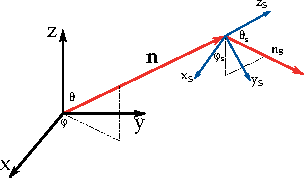
\includegraphics[width=0.5\textwidth]{frame-rot.pdf}
	\caption{Illustration of rotating the centre of mass frame to the lab frame. $\mathbf{n}$ is the direction vector of the photon before scattering, and $\mathbf{n_s}$ is the scattered direction vector. $\theta$ and $\varphi$ are the scattering angles. $z_s$ is in the same direction as $\mathbf{n}$.}
	\label{fig:labframerotate}
\end{figure}


\subsubsection*{Termination}\label{sec:terminator}

The final section of the \gls*{mcrt} algorithm is to check if it should be terminated. This is a simple check to see if there are any more photons to run.
If there are more photons to run then the algorithm goes back to the~\nameref{sec:photlaunch} section and continues from there.
If there are no more photons the algorithm terminates and any results are written out.


\subsubsection*{Scored Quantities}\label{sec:fluencecalc}

As~\gls*{mcrt} is a computational method, a wealth of information is able to be recorded during the simulation.
From the paths of individual photons, to average scattering angles and more.
However, it is not practical to record all this information for every simulation, as this would lead to inefficient simulations, and expensive data storage solutions.
Thus, for a given problem only the pertinent information is stored.

One important recorded variable is fluence.
Fluence is the number of photons entering a sphere per unit cross section area~\cite{rogers1990monte}.
In practice the average fluence per area is used,~\cref{eqn:jmean}, as this is easier to calculate in an~\gls*{mcrt} code.
Lucy showed that the average fluence per area is proportional to the sum of the path length through a volume~\cite{lucy1999computing}:

\begin{equation}
J_i = \frac{L}{NV_{\varsigma}}\sum l 
\label{eqn:jmean}
\end{equation}

\noindent Where:

\indent $J_i$ is the mean intensity such that the fluence is $\Phi=4\pi J$ [$W\ m^{-2}$];

\indent $L$ is the luminosity or power of the light source [$W$];

\indent $N$ is the total number of photon packets [-];

\indent $V_{\varsigma}$ is the volume of the $\varsigma^{th}$ voxel [$m^3$];

\indent and $l$ is the path length of a photon packet through the $\varsigma^{th}$ voxel [$m$]. 

\medskip

Most chapters in this thesis make use of~\cref{eqn:jmean} or modified versions of it as the main scored quantity, e.g. to determine absorbed energy.

Other common scored quantities are the exit location of a photon, the wavelength of an exiting photon or the distribution of photon packet absorption.

\subsection{Code Details}

This section describes the implementation of the \gls*{mcrt} and of the parallelisation the code.

\subsubsection*{Code}

All code in this thesis is written in modern Fortran\footnote{modern Fortran is considered anything past Fortran 95~\cite{metcalf2011modern}.}.
All subroutines and functions are contained in modules (with the exception of the main program---main.f90).
This is done to be able to ``hide'' data from subroutines and functions, and to arrange the code that relates to other parts of the code in the same file.
Having the code in modules also allows the use of runtime allocation of memory for arrays.
This enables the user to specify the size of arrays depending on the need of the user for the problem at hand.

Modules are classified into three different types: data, routines, and dependencies.
Data modules are modules that contain no function or routines, but store variables that can be accessed anywhere in the program when required.
Routine modules contain the subroutines and functions used in the code.
Finally dependency modules are the modules that have not been written by me, and thus the code depends upon them to run.

\Cref{fig:codegraph} show the relationship between the various modules, for a basic version of the \gls*{mcrt} as described in~\nameref{sec:algorithmMCRT}.

\medskip
\noindent Using~\cref{fig:codegraph} as a reference each module contains:

\noindent {\color{green}\textit{mcpolar.f90}} is the entry point of the code. It calls all other subroutines and functions, as well as setting up various variables and printing progress.

\noindent {\color{lightblue2}\textit{ch_opt}} is the module where the optical properties are set or changed.

\noindent {\color{lightblue2}\textit{gridset_mod}} is where the optical properties grid and voxel walls are set.

\noindent {\color{lightblue2}\textit{subs}} contains general purpose routines that are used in various different parts of the code.

\noindent {\color{lightblue2}\textit{writer_mod}} contains routines that write out the results of the simulation.

\noindent {\color{lightblue2}\textit{inttau2}} is the module that contains the routines that propagate the photon through the voxel grid.

\noindent {\color{lightblue2}\textit{sourceph_mod}} contains the routines that initialise the photon position and direction.

\noindent {\color{lightblue2}\textit{stokes_mod}} contains the routine that calculates the scattering direction after a scattering event.

\noindent {\color{red}\textit{iarray}} is a data module that contains all the arrays in the code.

\noindent {\color{red}\textit{constants}} is a data module that contains all the constants and filepaths needed in the code.

\noindent {\color{gray}\textit{ieee_arithmetic}} is an external dependency that gives various arithmetic checking routines such as is_nan().

\noindent {\color{lightblue2}\textit{vector_class}} is a module that contains the vector type, and all its associated operations such as cross and dot products of vectors.

\noindent {\color{red}\textit{photon_vars}} is a data module that contains the data pertaining to each photon, such as wavelength or energy.

\noindent Finally, {\color{red} \textit{opt_prop}} contains the data about the current optical properties such as the albedo and absorption coefficient.


\begin{figure}[!htbp]
	\centering
	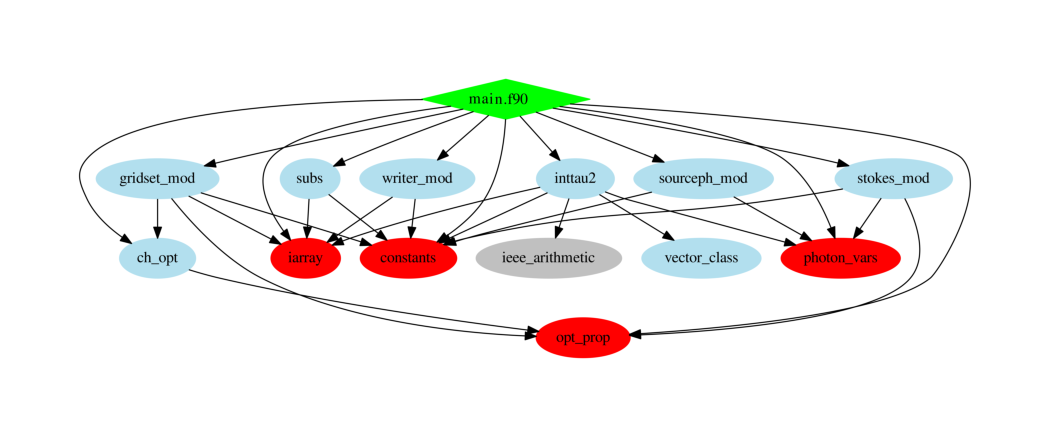
\includegraphics[width=0.95\textwidth]{graph-code.pdf}
	\caption{Source code hierarchy, showing the relationship between different modules. Green is the entry point for the simulation. Red are the data modules, light blue are the routine modules, and grey are the external dependencies.}
	\label{fig:codegraph}
\end{figure}



\subsection*{Parallelisation of the MCRT Algorithm}\label{sec:parasec}

As mentioned in the previous sections, \gls*{mcrt} can be computationally intensive, especially when dealing with highly scattering mediums. Fluorescence can also cause simulations times to drastically increase as photons are no longer ``killed'' off, but rather re-emitted at a new wavelength. Other optical processes such as Raman scattering are highly unlikely events, which again can lead to a dramatic increase in simulation times, as many photons are required to be simulated to get ``good'' statistics.

Fortunately \gls*{mcrt} is classed as an ``embarrassingly parallel'' problem\footnote{However, this is not true for all \gls*{mcrt} applications. For example, using the Bjorkman $\&$ Wood~\cite{bjorkman2001radiative} immediate temperature corrections method, turns \gls*{mcrt} into a different class of parallel problem~\cite{robitaille2011hyperion}.}.
This means that it is trivial to parallelise in comparison to other algorithms. 
The reason that \gls*{mcrt} is classed as ``embarrassingly parallel'', is that the algorithm can be split up onto separate processors, with little need for communication between them. 
In reality this means that $n$ copies of the algorithm can run on $n$ cores in a processor, with communication taking place at the start and end of each simulation run. 

All the code in this thesis is parallelised using \gls*{mpi}~\cite{gropp2014using,gropp2014usingadv}, with the only communication taking place at the end, where the results are collated on to all processes.
The one exception to this is in~\cref{chap:ablation}, where the heat diffusion calculation needs communication between the processes during the calculation.

The parallel efficiency of a code depends on the problem and the number of photon packets run.
To determine the speedup of a given problem, Amdahl's law is used~\cite{amdahl1967validity}:

\begin{equation}
speedup = \frac{1}{(1-P)+P/N}
\end{equation}

Where $P$ is the fraction of the code that is parallel, and N is the number of cores the code is run on.
The consequence of Amdahl's law is as $N$ tends to infinity the speedup tends to a maximum:

\begin{equation}
speedup_{max}=\frac{1}{1-P}
\end{equation}

The value of P varies from problem to problem and the number of photon packets run.
\Cref{fig:paratest} shows the results of the profiling of the code, for various numbers of cores.
This test consisted of running the same number of photons, in a highly scattering medium of size $2~cm^3$.
This yielded a $P$ of $0.999010 \pm 0.000045$ and a maximum speedup of 1010.1.


\begin{figure}[!htbp]
	\centering
	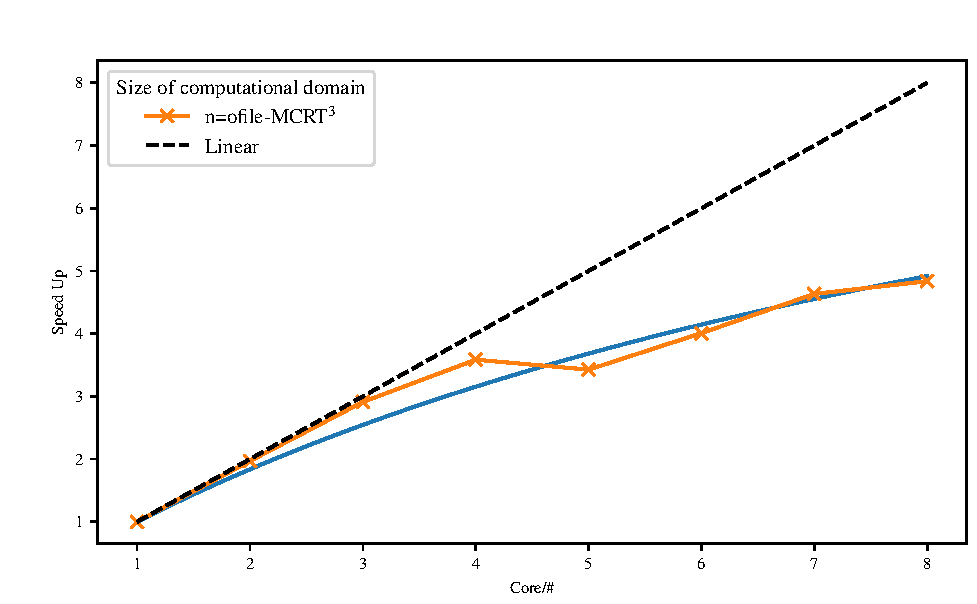
\includegraphics[width=0.75\textwidth]{profile-mcrt.pdf}
	\caption{Performance of the parallelisation of the MCRT code using MPI.}
	\label{fig:paratest}
\end{figure}


\FloatBarrier
\section{Validation of MCRT Code}\label{sec:validation}

As the Monte Carlo method is an algorithm that depends upon random numbers, it is sometimes hard to ensure the correct result is obtained.
Or to put it another way:
\medskip

``Monte Carlo is easy to do wrong!'' G.W. Collins III~\cite{bjormaneasymonte}

\medskip

Thus, the code has to be validated against various theoretical/experimental and other simulations, to determine whether the results are correct.

The main benchmark of the~\gls*{mcrt} code is a comparison against an expression for fluence as a function of depth~\cite{gardner1993fluorescence}.
This expression has also been fitted to by other~\gls*{mcrt} simulations~\cite{jacques1993photobleaching}.

\begin{equation}
\Psi(z)=\Psi_0(C_1e^{-k_1z/\delta}-C_2e^{-k_2z/\delta})
\label{eqn:jacqmatch}
\end{equation}

\noindent Where:

\indent $\Psi(z)$ is the penetration of the incident light, or equivalently the fluence rate [$W\ cm^{-2}$];

\indent $\Psi_0$ is a normalisation constant [$W\ cm^{-2}$];

\indent $C_n$ and $k_n$ are fitted coefficients [-];

\indent and $\delta$ is the optical penetration depth, defined as $\delta=1/\sqrt{3\mu_a(\mu_a+\mu_s(1-g))}$, [$cm$].

\medskip

Jacques \textit{et al.}, in their simulation used two different wavelengths, 420~nm and 630~nm.
The medium in the simulation is an infinitely wide slab with a depth of 1~cm, with uniform optical properties. 
The medium has a refractive index of 1.38.
The $g$ value is in the range 0.7 --- 0.9, and the optical properties are as in~\cref{tab:jacqprops}.

\begin{table}[!ht]
\begin{tabular}{llllllll}
                                   & \multicolumn{1}{c}{{\ul Absorption}} & \multicolumn{1}{c}{{\ul Scattering}}    & \multicolumn{4}{c}{{\ul Penetration}}          &             \\
\multicolumn{1}{l|}{Wavelength/nm} & \multicolumn{1}{l|}{$\mu_a$/$cm^{-1}$} & \multicolumn{1}{l|}{$\mu_s(1-g)/cm^{-1}$} & C1   & k1   & C2   & \multicolumn{1}{l|}{k2}   & $\delta/cm$ \\ \hline
\multicolumn{1}{l|}{420}           & \multicolumn{1}{l|}{1.8}             & \multicolumn{1}{l|}{82}                 & 5.76 & 1.00 & 1.31 & \multicolumn{1}{l|}{10.2} & 0.047       \\
\multicolumn{1}{l|}{630}           & \multicolumn{1}{l|}{0.23}            & \multicolumn{1}{l|}{21}                 & 6.27 & 1.00 & 1.18 & \multicolumn{1}{l|}{14.4} & 0.261      
\end{tabular}
\caption{Table of optical properties and determined coefficients from Jacques \textit{et al.}~\cite{jacques1993photobleaching}.}
\label{tab:jacqprops}
\end{table}

Using these values Jacques \textit{et al.} calculated values for $C_1,\ C_2,\ k_1$ and $k_2$ using their \gls*{mcrt} code.
The above optical properties and medium dimensions\footnote{The infinitely wide slab is implemented so that when a photon leaves one of the sides of the voxel grid, it is moved to the other side of the grid, retaining its original direction vectors.} are recreated in the code and a value of 0.9 was chosen for $g$.
8 million photons were run for the simulation.
This yielded the result as in~\cref{fig:matchjacq}.

\begin{figure}[!htbp]
	\centering
	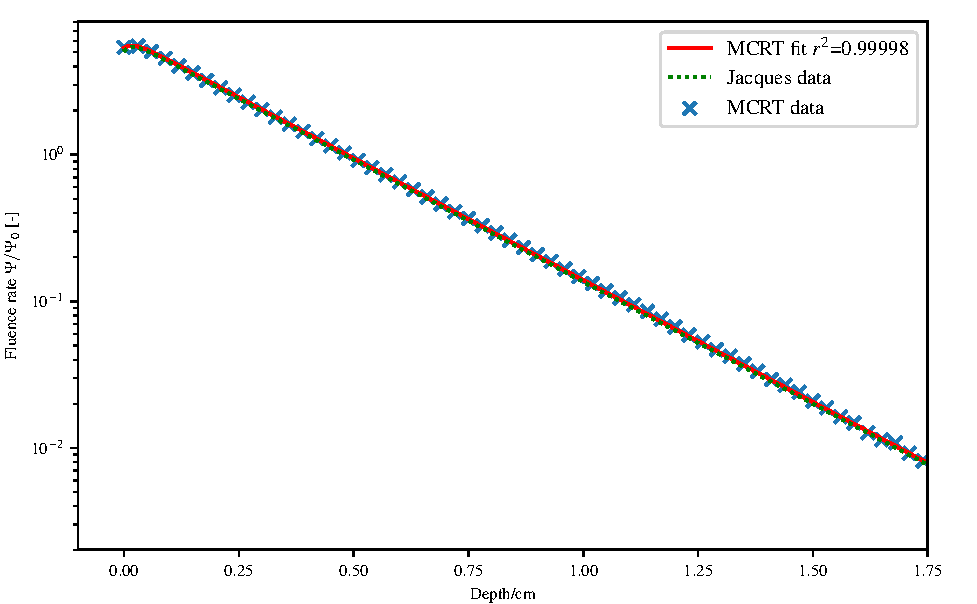
\includegraphics[width=0.75\textwidth]{validation-jacques.pdf}
	\caption{Figure shows the fluence as a function of depth. Figure also shows comparison to the Jacques MCRT simulation and the MCRT as described in this chapter.}
	\label{fig:matchjacq}
\end{figure}


Fitting~\cref{eqn:jacqmatch} to the data calculated by our~\gls*{mcrt} code for $630~nm$, gave: $C_1 = 6.425$, $C_2=1.083$, $k_1=1.0$, and $k_2=12.966$.
For $420~nm$ gave: $C_1 = 5.600$, $C_2=0.838$, $k_1=1.003$, and $k_2=9.846$.
These are in good agreement (within code differences) with Jacques \textit{et al.} results.

\section{Conclusion}

There are various methods available to model the radiative transport equation.
\Gls*{mcrt} is the most flexible of the methods available, allowing arbitrary geometries, light sources, multiple anisotropic scattering, and various microphysics to be modelled.
This chapter presented an overview of the \gls*{mcrt} algorithm that will be the basis of the results presented in the following chapters.
The code described in this chapter is based upon K. Wood's \gls*{mcrt} code for light propagation in galactic dust clouds.
It has been rewritten in modern Fortran and adapted so that the code can model biological tissue so that the code can be applied to various medical and biophotonic problems.
The optical properties required in a \gls*{mcrt} simulation have been discussed, and will be utilised to subsequent chapters.
A description of how the code has been parallelised and validated against a standard literature code has also been presented.
